\documentclass{beamer}
\RequirePackage{luatex85}
\include{../style/cours-style.sty}

% Title
\title{Scripting - Bachelor CSI}
\author{Christophe Brun}
\institute{Campus Saint-Michel IT}
\date{25 juin 2024}
\beamertemplatenavigationsymbolsempty

\titlegraphic{
    \bigbreak
    
\includegraphics[width=2cm]{image/logo-papit}
    
\includegraphics[width=2cm]{image/logo-campus-saint-michel-it}
}
\begin{document}

    \begin{frame}
        \titlepage
        \bigbreak
        %\centering
        %\url{https://github.com/St-Michel-IT/data-security/}
    \end{frame}

    \begin{frame}{Table des matières}
        \tableofcontents
    \end{frame}


    \section{Programme du module}\label{sec:programme-du-module}
    \begin{frame}{Scripting}{Programme et compétence}
        \begin{enumerate}
            \item Gestion des arguments d’un script
            \item Gestion des erreurs
            \item Librairies utiles pour interroger le système et le modifier
            \item Introduction aux Regex
            \item SSH et les clés RSA
            \item Se connecter à des serveurs
            \item Automatiser des installations de serveurs
            \item Monitoring de ressources
        \end{enumerate}
        Compétence~:
        \bigbreak
        Automatiser des tâches d’administration système à l’aide d’un langage de script.
    \end{frame}

    \begin{frame}{Intervenant sur le module Scripting}{Christophe Brun, conseil en développement informatique}

        \begin{columns}
            \column{0.7\textwidth}
            \begin{itemize}
                \item 2\textsuperscript{nde} année d'intervenant à Saint-Michel \emoji{star-struck}.

                \item 7 ans de conseil en développement au sein d'SSII~.

                \item 7 ans de conseil en développement à mon compte \href{https://papit.fr}{PapIT}.

                \item Passionné~!
                \bigbreak
                \begin{columns}
                    \column{0.5\textwidth}
                    \centering
                    
\includegraphics[width=3cm]{image/logo-uppa}
                    \column{0.5\textwidth}
                    \centering
                    
\includegraphics[width=3cm]{image/logo-universite-bordeaux}
                \end{columns}
            \end{itemize}
            \column{0.3\textwidth}
            \centering
            
\includegraphics[width=5cm]{image/trombine-christophe}
        \end{columns}
    \end{frame}


    \section{VM management}\label{sec:vm-management}
    \begin{frame}{VM management}
        \bigbreak
        \centering
        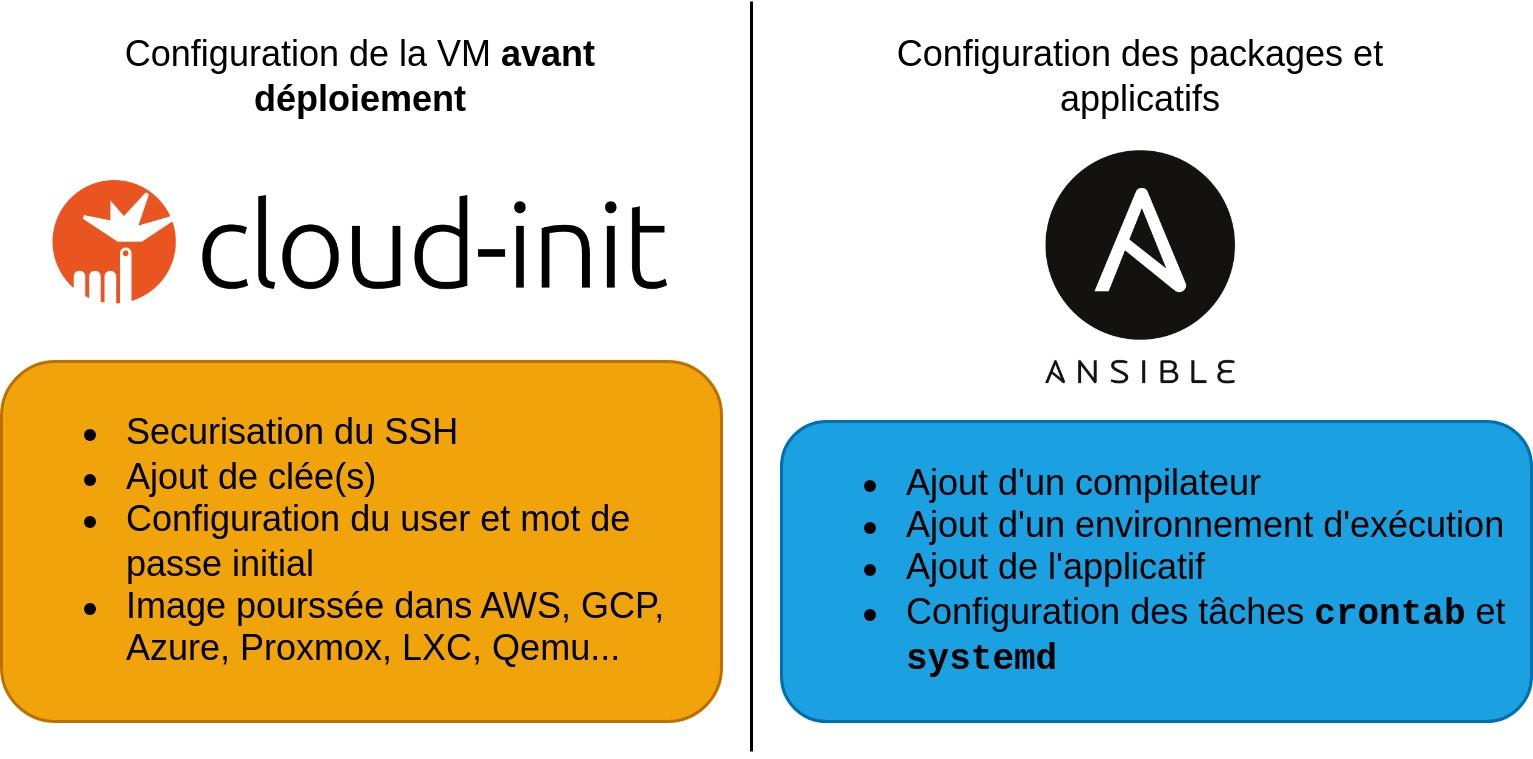
\includegraphics[width=12cm]{image/cloud-init-vs-ansible}
    \end{frame}


    \section{Préparation de la VM}\label{sec:prepare-vm}
    \begin{frame}{Configuration du SSH}{Sécurisation du SSH avec la cryptographie asymétrique}
        \begin{footnotesize}
            Pourquoi est-ce plus sécure d'utiliser une clé SSH plutôt qu'un mot de passe~?
            \bigbreak
            Quels algorithmes et taille de clé sont recommandés~?
            \pause
            \bigbreak
            Sur le site \url{https://jadaptive.com/ssh-key-management/the-benefits-of-ssh-key-authentication/} on trouve~:
            \begin{columns}
                \begin{column}{0.6\textwidth}
                    \begin{itemize}
                        \item Le mot de passe doit être communiqué à chaque connexion, il est donc plus vulnérable à une interception/sniffing/MITHM~.
                        La clé privée reste sur le client, elle n'est pas communiquée.
                        \item La clé SSH est plus complexe à deviner qu'un mot de passe.
                        \item On peut automatiser des taches depuis la machine cliente avec la clé SSH~.
                    \end{itemize}
                \end{column}
                \begin{column}{0.4\textwidth}
                    \centering
                    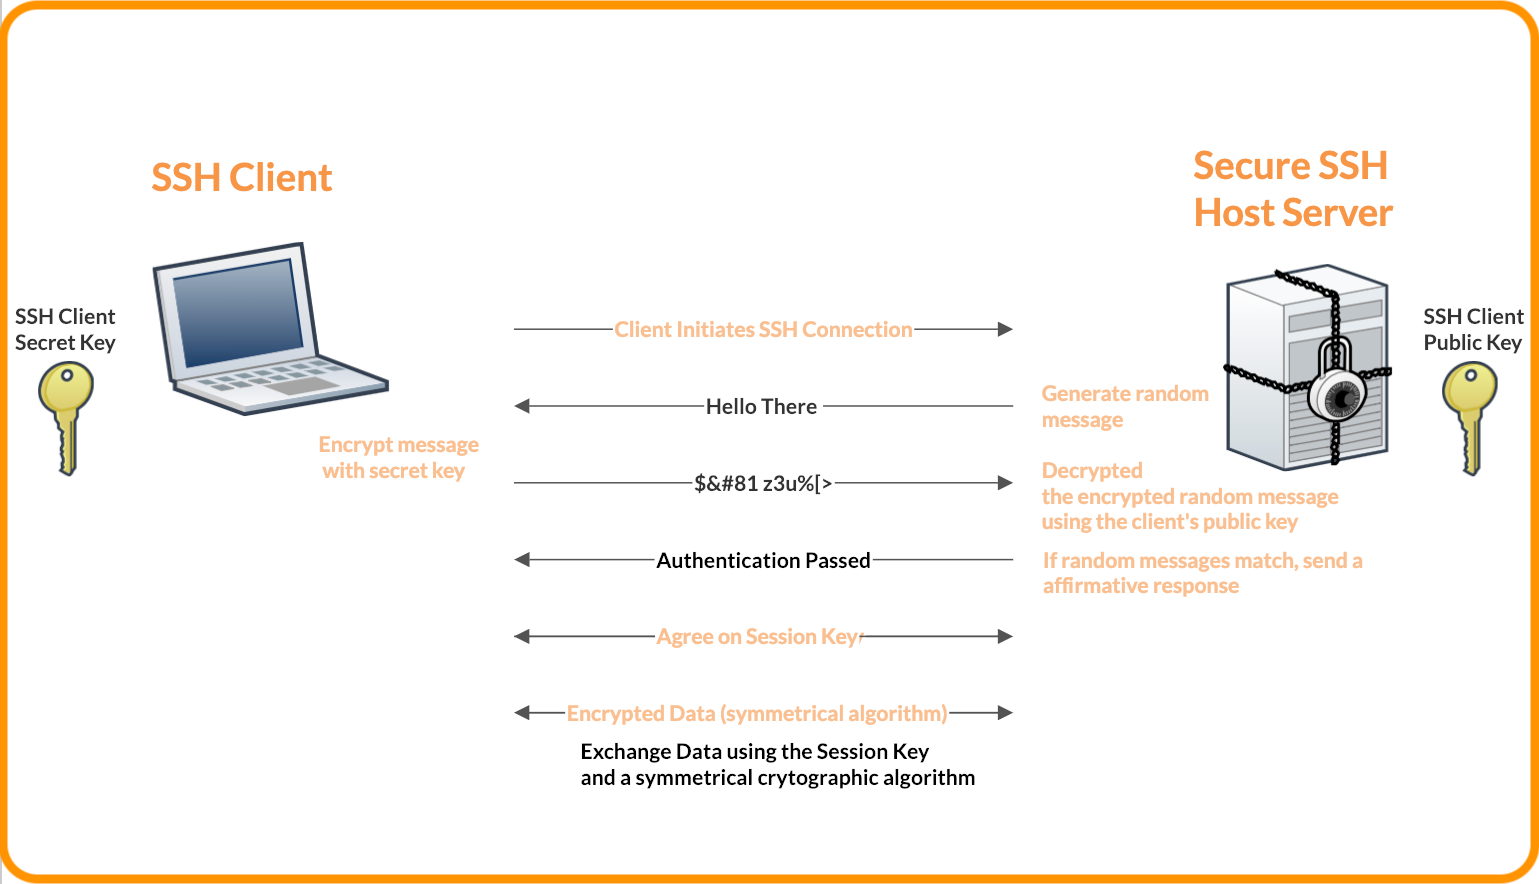
\includegraphics[width=5cm]{image/ssh-key-diagram} \\ Foxpass\footnotemark \\
                \end{column}
            \end{columns}
            \footnotetext{Learn SSH Keys in Minutes, \url{https://www.foxpass.com/blog/learn-ssh-keys-in-minutes/}}
        \end{footnotesize}
    \end{frame}

    \begin{frame}[fragile]{Configurer le SSH}{Une des solutions (commande à exécuter sur la VM)}
        Commande pour configurer la VM~:
        \begin{lstlisting}[language=bash][fragile]
# Configure SSH
sed -i '/PermitRootLogin/d' /etc/ssh/sshd_config
echo "PermitRootLogin no" >> /etc/ssh/sshd_config
sed -i '/PasswordAuthentication/d' /etc/ssh/sshd_config
echo "PasswordAuthentication no" >> /etc/ssh/sshd_config
# Restart SSH with the new configuration
sudo systemctl restart sshd
# Create the .ssh directory and the authorized_keys file
mkdir -p ~/.ssh
touch ~/.ssh/authorized_keys
# Add the public key to the authorized_keys file
echo "ssh-rsa AAAAB3NzaC1yc2EAAAADAQABAAABgQDQ8z4... chrichri@localhost" >> ~/.ssh/authorized_keys
        \end{lstlisting}
        \begin{columns}
            \column{0.5\textwidth}
            Expliquer chaque commande.
            \column{0.5\textwidth}
            \begin{center}
                
\includegraphics[width=2cm]{image/funny-key}
            \end{center}
        \end{columns}
    \end{frame}

    \begin{frame}{Cloud-init\footnote{Cloud-init, The standard for customising cloud instances, \url{https://cloud-init.io/}}}
        Cloud-init est un outil qui permet de configurer une VM lors de son déploiement.
        \bigbreak
        Il est possible de configurer~:
        \begin{itemize}
            \item Le nom de la machine.
            \item Les utilisateurs.
            \item Les clés SSH.
            \item Les scripts à exécuter.
        \end{itemize}
        Il est compatible avec la plupart des hyperviseurs et \textit{cloud providers}.
        \bigbreak
        \centering
        
\includegraphics[width=10cm]{image/cloud-init}
    \end{frame}

    \begin{frame}{Cloud-init}{Déploiement d'une VM vierge sécurisée}
        Exercice \execcounterdispinc{}~:
        Avec Cloud-init dans un premier script Shell~:
        \begin{itemize}
            \item Restreindre l'accès à la VM au SSH avec une clé SSH, aucun mot de passe.
            \item Pas de root en SSH
            \item Créez un user pour un de vos camarades.
            \item Donner un Shell \lstinline{bash} par défaut.
        \end{itemize}
        Dans un second script Shell~:
        \begin{itemize}
            \item Lancer la VM
        \end{itemize}
        Utiliser des images cloud pour Qemu de chez Ubuntu ou Rocky Linux.
    \end{frame}


    \section{Ansible}\label{sec:ansible}

    \begin{frame}{Automatisation de la configuration avec Ansible}{Définition\footnote{Ansible Community Documentation, \url{https://docs.ansible.com/ansible/latest/getting_started/index.html}}}
        Ansible est un outil d'automatisation de la configuration des machines physiques ou virtuelles.
        Il permet de définir des \textquote{playbooks} qui décrivent une configuration à appliquer aux machines qui sont dans l'\textquote{inventory} .
        \bigbreak
        \centering
        
\includegraphics[width=3cm]{image/logo-ansible}
    \end{frame}

    \begin{frame}[fragile]{Automatisation de la configuration avec Ansible}{Exemple d'inventaire}
        Pour accéder à la VM créée précédemment dans Qemu, il faut définir un inventaire avec les données dont on aurait besoin pour y accéder en SSH~.
        \begin{lstlisting}[language=bash,basicstyle=\ttfamily\tiny]
$ ssh chrichri@localhost -p 5022 -v -i /home/chrichri/Documents/Campus-St-Michel-IT/production-deployment/virt-ubuntu
        \end{lstlisting}
        La commande ci-dessus, devient dans l'inventaire (on peut créer des variables)~:
        \begin{lstlisting}[language=bash,basicstyle=\ttfamily\tiny]
[gunicorn]
localhost:5022 ansible_ssh_private_key_file=/home/chrichri/Documents/Campus-St-Michel-IT/production-deployment/virt-ubuntu ansible_ssh_user=chrichri
        \end{lstlisting}
        On utilise le module \lstinline{ping} pour vérifier que l'accès SSH est correctement configuré.
        \begin{lstlisting}[language=bash,basicstyle=\ttfamily\tiny]
$ ansible gunicorn -m ping -i inventory.ini
localhost | SUCCESS => {
    "ansible_facts": {
        "discovered_interpreter_python": "/usr/bin/python3"
    },
    "changed": false,
    "ping": "pong"
}
        \end{lstlisting}
    \end{frame}

    \begin{frame}{Automatisation de la configuration avec Ansible}{Aucune installation côté client\emoji{heart}}
        Pourquoi Ansible n'a aucun client sur les machines de l'inventaire~?
        \bigbreak
        \centering
        
\includegraphics[width=5cm]{image/question-mark-on-a-blank-background}
        \bigbreak
        \pause
        \flushleft
        Avec le seul accès SSH, il exécute les commandes qu'il faut.
        Il est agnostique à l'OS~!
    \end{frame}

    \begin{frame}[fragile]{Automatisation de la configuration avec Ansible}{Exemple de \textquote{playbook}}
        Qu'a-t-on installé sur un Ubuntu \textit{cloud image} comme package(s) pour pouvoir exécuter l'application gunicorn Hello World~?
        \pause
        % With apt, packages python3-gunicorn
        \begin{lstlisting}[language=bash]
sudo apt-get install python3-gunicorn
        \end{lstlisting}
        Commande qui devient dans un playbook Ansible \lstinline{gunicorn.yml}~:
        \begin{lstlisting}
---
- name: gunicorn
  hosts: gunicorn
  become: yes # Run as root
  tasks:
  - name: Install gunicorn
    apt:
      name: gunicorn # Le package à installer
      state: present
        \end{lstlisting}
        À lancer avec la commande~:
        \begin{lstlisting}[language=bash]
$ ansible-playbook -i inventory.ini gunicorn.yml
        \end{lstlisting}
    \end{frame}

    \begin{frame}[fragile]{Automatisation de la configuration avec Ansible}{Exemple de \textquote{playbook}}
        Le résultat de l'exécution du playbook \lstinline{gunicorn.yml}~:
        \begin{lstlisting}[language=bash]
$ ansible-playbook -i inventory.ini gunicorn.yml
...
localhost                  : ok=2    changed=1    unreachable=0    failed=0    skipped=0    rescued=0    ignored=0

$ ansible-playbook -i inventory.ini gunicorn.yml
...
localhost                  : ok=2    changed=0    unreachable=0    failed=0    skipped=0    rescued=0    ignored=0
        \end{lstlisting}
        À la première exécution, le package est installé, à la seconde il est déjà installé, aucun changement.
    \end{frame}

    \begin{frame}[fragile]{Automatisation de la configuration avec Ansible}{Commande pour exécuter un programme}
        Une fois les dépendances requises installées, on peut exécuter un programme avec le module \lstinline{shell}~.
        \bigbreak
        S’il faut copier un ou plusieurs fichiers, on peut utiliser le module \lstinline{copy}~.
        \bigbreak
        Par exemple~:
        \begin{lstlisting}
---
- hosts: gunicorn # Groupe de host de l'inventory
  vars:
  - EXEC_ABS_PATH: /home/chrichri/helloworld # Utilisé 2 fois donc dans une variable
...
  - name: Copy Application
    copy:
      src: /home/chrichri/Documents/Campus-St-Michel-IT/production-deployment/helloworld/build/helloworld # Le build de ma machine
      dest: "{{ EXEC_ABS_PATH }}"

  - name: Run Application
    shell: nohup {{ EXEC_ABS_PATH }} & # nohup pour exécuter en arrière plan
        \end{lstlisting}
    \end{frame}

    \begin{frame}{Automatisation de la configuration avec Ansible}{La Ansible Galaxy}
        Comme souvent, inutile de tout recoder.
        Ansible est modulaire grâce aux \textquote{roles} et aux \textquote{playbooks} qui sont eux-mêmes des modules\footnote{Roles, \url{https://docs.ansible.com/ansible/latest/playbook_guide/playbooks_reuse_roles.html}}.
        \bigbreak
        La communauté Ansible a packagé des modules et des playbooks pour les tâches les plus courantes\footnote{Ansible Galaxy, \url{https://galaxy.ansible.com/ui/}}.
        Ils sont disponibles sur la \href{https://galaxy.ansible.com/}{Ansible Galaxy}.
        Et peuvent être installés avec la commande \lstinline{ansible-galaxy install <module>}, commande issue du package \lstinline{ansible-core}.
    \end{frame}

    \begin{frame}{Automatisation de la configuration avec Ansible}{Ansible et Windows}
        Sur la machine hôte, on ne peut l'installer que depuis un WSL~.
        \begin{dangercolorbox}
            Si la machine cliente est un Windows, attention au package manager et aux séparateurs de chemin, voir \url{https://docs.ansible.com/ansible/latest/os_guide/windows_usage.html}.
        \end{dangercolorbox}
        \bigbreak
        \centering
        
\includegraphics[width=5cm]{image/broken-windows} \\ L'idéal reste quand même de ne pas utiliser Windows\ldots \\
    \end{frame}

    \begin{frame}{Automatisation de la configuration avec Ansible}{Exercice \execcounterdispinc{}}
        En utilisant la VM crée à l'exercice précédent, configurer un inventaire et un playbook pour installer l'application Spring Boot.
        \bigbreak
        Vous pouvez vous aider du \href{https://spring.io/guides/gs/spring-boot}{tutoriel officiel}.
        \bigbreak
        \centering
        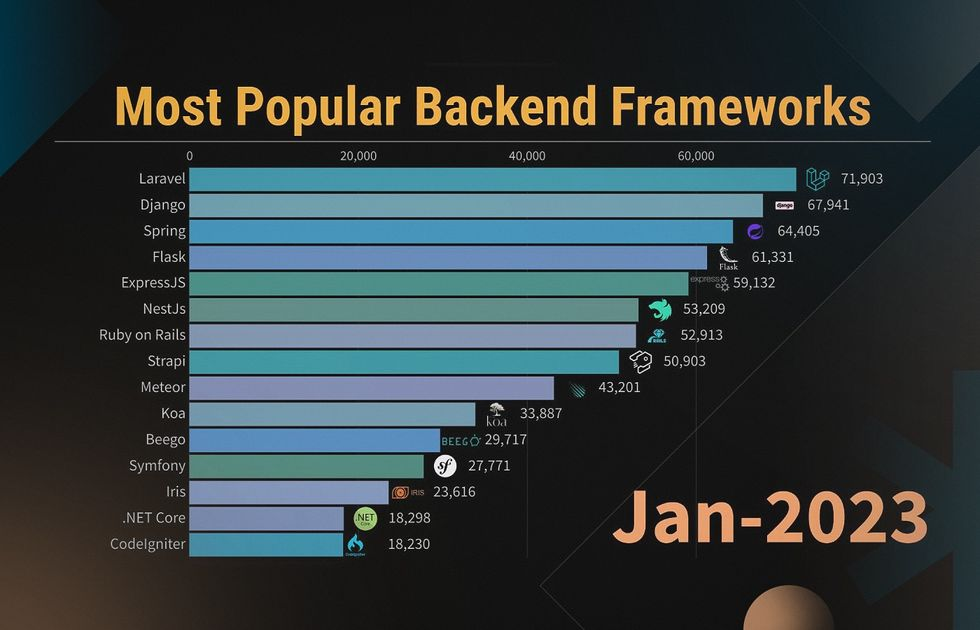
\includegraphics[width=8cm]{image/most-popular-backend}
    \end{frame}

    \begin{frame}{Automatisation de la configuration avec Ansible}{Solution à l'exercice précédent}
        De nombreuses solutions sont valides.
        Mais avec Java il est plus simple de profiter du \textquote{Write once, run anywhere}.
        \bigbreak
        Ce n'est donc pas obliger d'utiliser un système de build comme Maven ou Gradle sur la VM, Java suffit pour exécuter une JAR~.
        \bigbreak
        Une JAR (Java ARchive) est un exécutable qui contient toutes les classes zippées et qui se lance avec \lstinline{java -jar <JAR file>}.
        Il suffit donc d'installer Java sur la JVM~.
    \end{frame}

    \begin{frame}[fragile]{Automatisation de la configuration avec Ansible}{Solution à l'exercice précédent}
        Par exemple, une solution avec uniquement Java 17~:
        \begin{lstlisting}[basicstyle=\ttfamily\tiny]
---
- hosts: gunicorn
  vars:
  - JAR_DEST_PATH: /home/chrichri/helloworld-0.0.1-SNAPSHOT.jar
  become: yes
  tasks:
  - name: Install Java 17
    apt:
      name: openjdk-17-jdk
      state: present

  - name: Copy Spring Boot Application
    copy:
      src: /home/chrichri/Documents/Campus-St-Michel-IT/production-deployment/helloworld/build/libs/helloworld-0.0.1-SNAPSHOT.jar
      dest: "{{ JAR_DEST_PATH }}"

  - name: Run Spring Boot Application
    shell: nohup java -jar {{ JAR_DEST_PATH }} &
        \end{lstlisting}
    \end{frame}


    \section{Licence CC}\label{sec:licence}

    \begin{frame}{Licence}{Licence Creative Commons}
        Support de cours sous licence Creative Commons BY-NC-ND~.
        \bigbreak
        Vous pouvez donc, partager, copier, distribuer le document.
        \bigbreak
        Attribution requise à PapIT SASU - Pas d’utilisation commerciale - Pas de modification
        \bigbreak
        \centering
        
\includegraphics[width=5cm]{image/by-nc-nd-logo}
    \end{frame}
\end{document}
